% 1) Title
% 2) Date
% 3) Location
% 4) Present
% 5) Picture
% 6) Start Time
% 7) Stop Time
\insertmeeting 
	{Multimedia Maze} 
	{09/01/21}
	{Hagerty High School}
	{Annika, Falon, Samantha}
	{Images/RobotPics/robot.jpg}
	{3:30}
  {4:30}
	
\hhscommittee{Multimedia}
\noindent\hfil\rule{\textwidth}{.4pt}\hfil
\subsubsection*{Goals}
\begin{itemize}
    \item Future plans for communications such as social media posts, coming up with outreach ideas that we can work on
\end{itemize} 

\noindent\hfil\rule{\textwidth}{.4pt}\hfil

\subsubsection*{Accomplishments}
After the program meeting we worked on planing for new social media posts and future ideas on outreach. Ms. Po helped us and discussed with us the school’s goal for inclusion at Hagerty. Her words inspired us to come up with some other ideas for outreach and how we could show inclusion within our team and in our community. Multimedia is currently working on Team member takeover posts that will show what each member on the team is all about and how they contribute to the making of 4717. We brainstormed some of the things that we had to get done for a while such as sponsor letters. We also wrote some stuff that we had for outreach and ideas for communication that could bring robotics and STEM closer to the community. Not only that, but it would be cool to show that our team likes to have fun, so we even spent some time to come up with some team bonding activities we could do in the future. All in all, we simply brainstormed plans that we could make for the team throughout the season and posts for our social media. 


\begin{figure}[ht]
\centering
  
\includegraphics[width=0.95\textwidth]{Meetings/September/09-01-21/1.jpeg}
  \caption{Our plans for outreach}
  \label{fig:090121_1}
\end{figure}

\hhscommittee{Hardware}
\noindent\hfil\rule{\textwidth}{.4pt}\hfil
\subsubsection*{Goals}
\begin{itemize}
    \item Teach 4227 members CAD basics
		\item Get to know 4227 members better

\end{itemize} 

\noindent\hfil\rule{\textwidth}{.4pt}\hfil

\subsubsection*{Accomplishments}
Today was our sister team, 4227 metalmorphosis’ first full robotics meeting. This would be the first time they would start working on robotics related things, and today they started with CAD. A few meetings ago they created onshape accounts, but they hadn’t begun learning it yet. In order to help them learn, several members of our hardware committee went to help them learn. We started out by giving a quick rundown of what CAD is and the basics of how it works. We then broke off and worked one on one with 4227 members, taking turns so everyone had an opportunity to learn.  Everyone got to try to make the first letter of their name, with some help from us 4717 members (image 1 and 2). This allowed them to learn how to make sketches, extrudes, chamfer, and fillets, all tools that we use regularly when designing our robots. For some of the 4227 members that were more interested in working with CAD in the future, we went into a bit more depth, showing them how to create assemblies and insert standard content, like screws and nuts (image 3). Overall they were able to make good progress in learning CAD and should be better prepared for the upcoming season.

\begin{figure}[ht]
\centering
\begin{minipage}[b]{.50\textwidth}
  \centering
  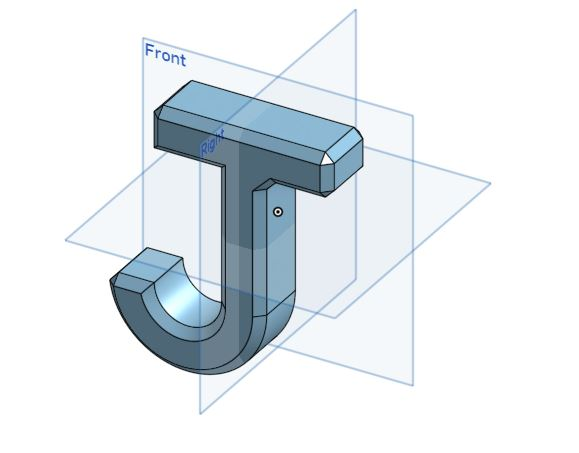
\includegraphics[width=0.8\textwidth]{Meetings/September/09-01-21/9-1-21_Program_Image1 - Nathan Forrer.JPG}
  \caption{The J we created in CAD}
  \label{fig:090121_1}
\end{minipage}%
\hfill%
\begin{minipage}[b]{.50\textwidth}
  \centering
  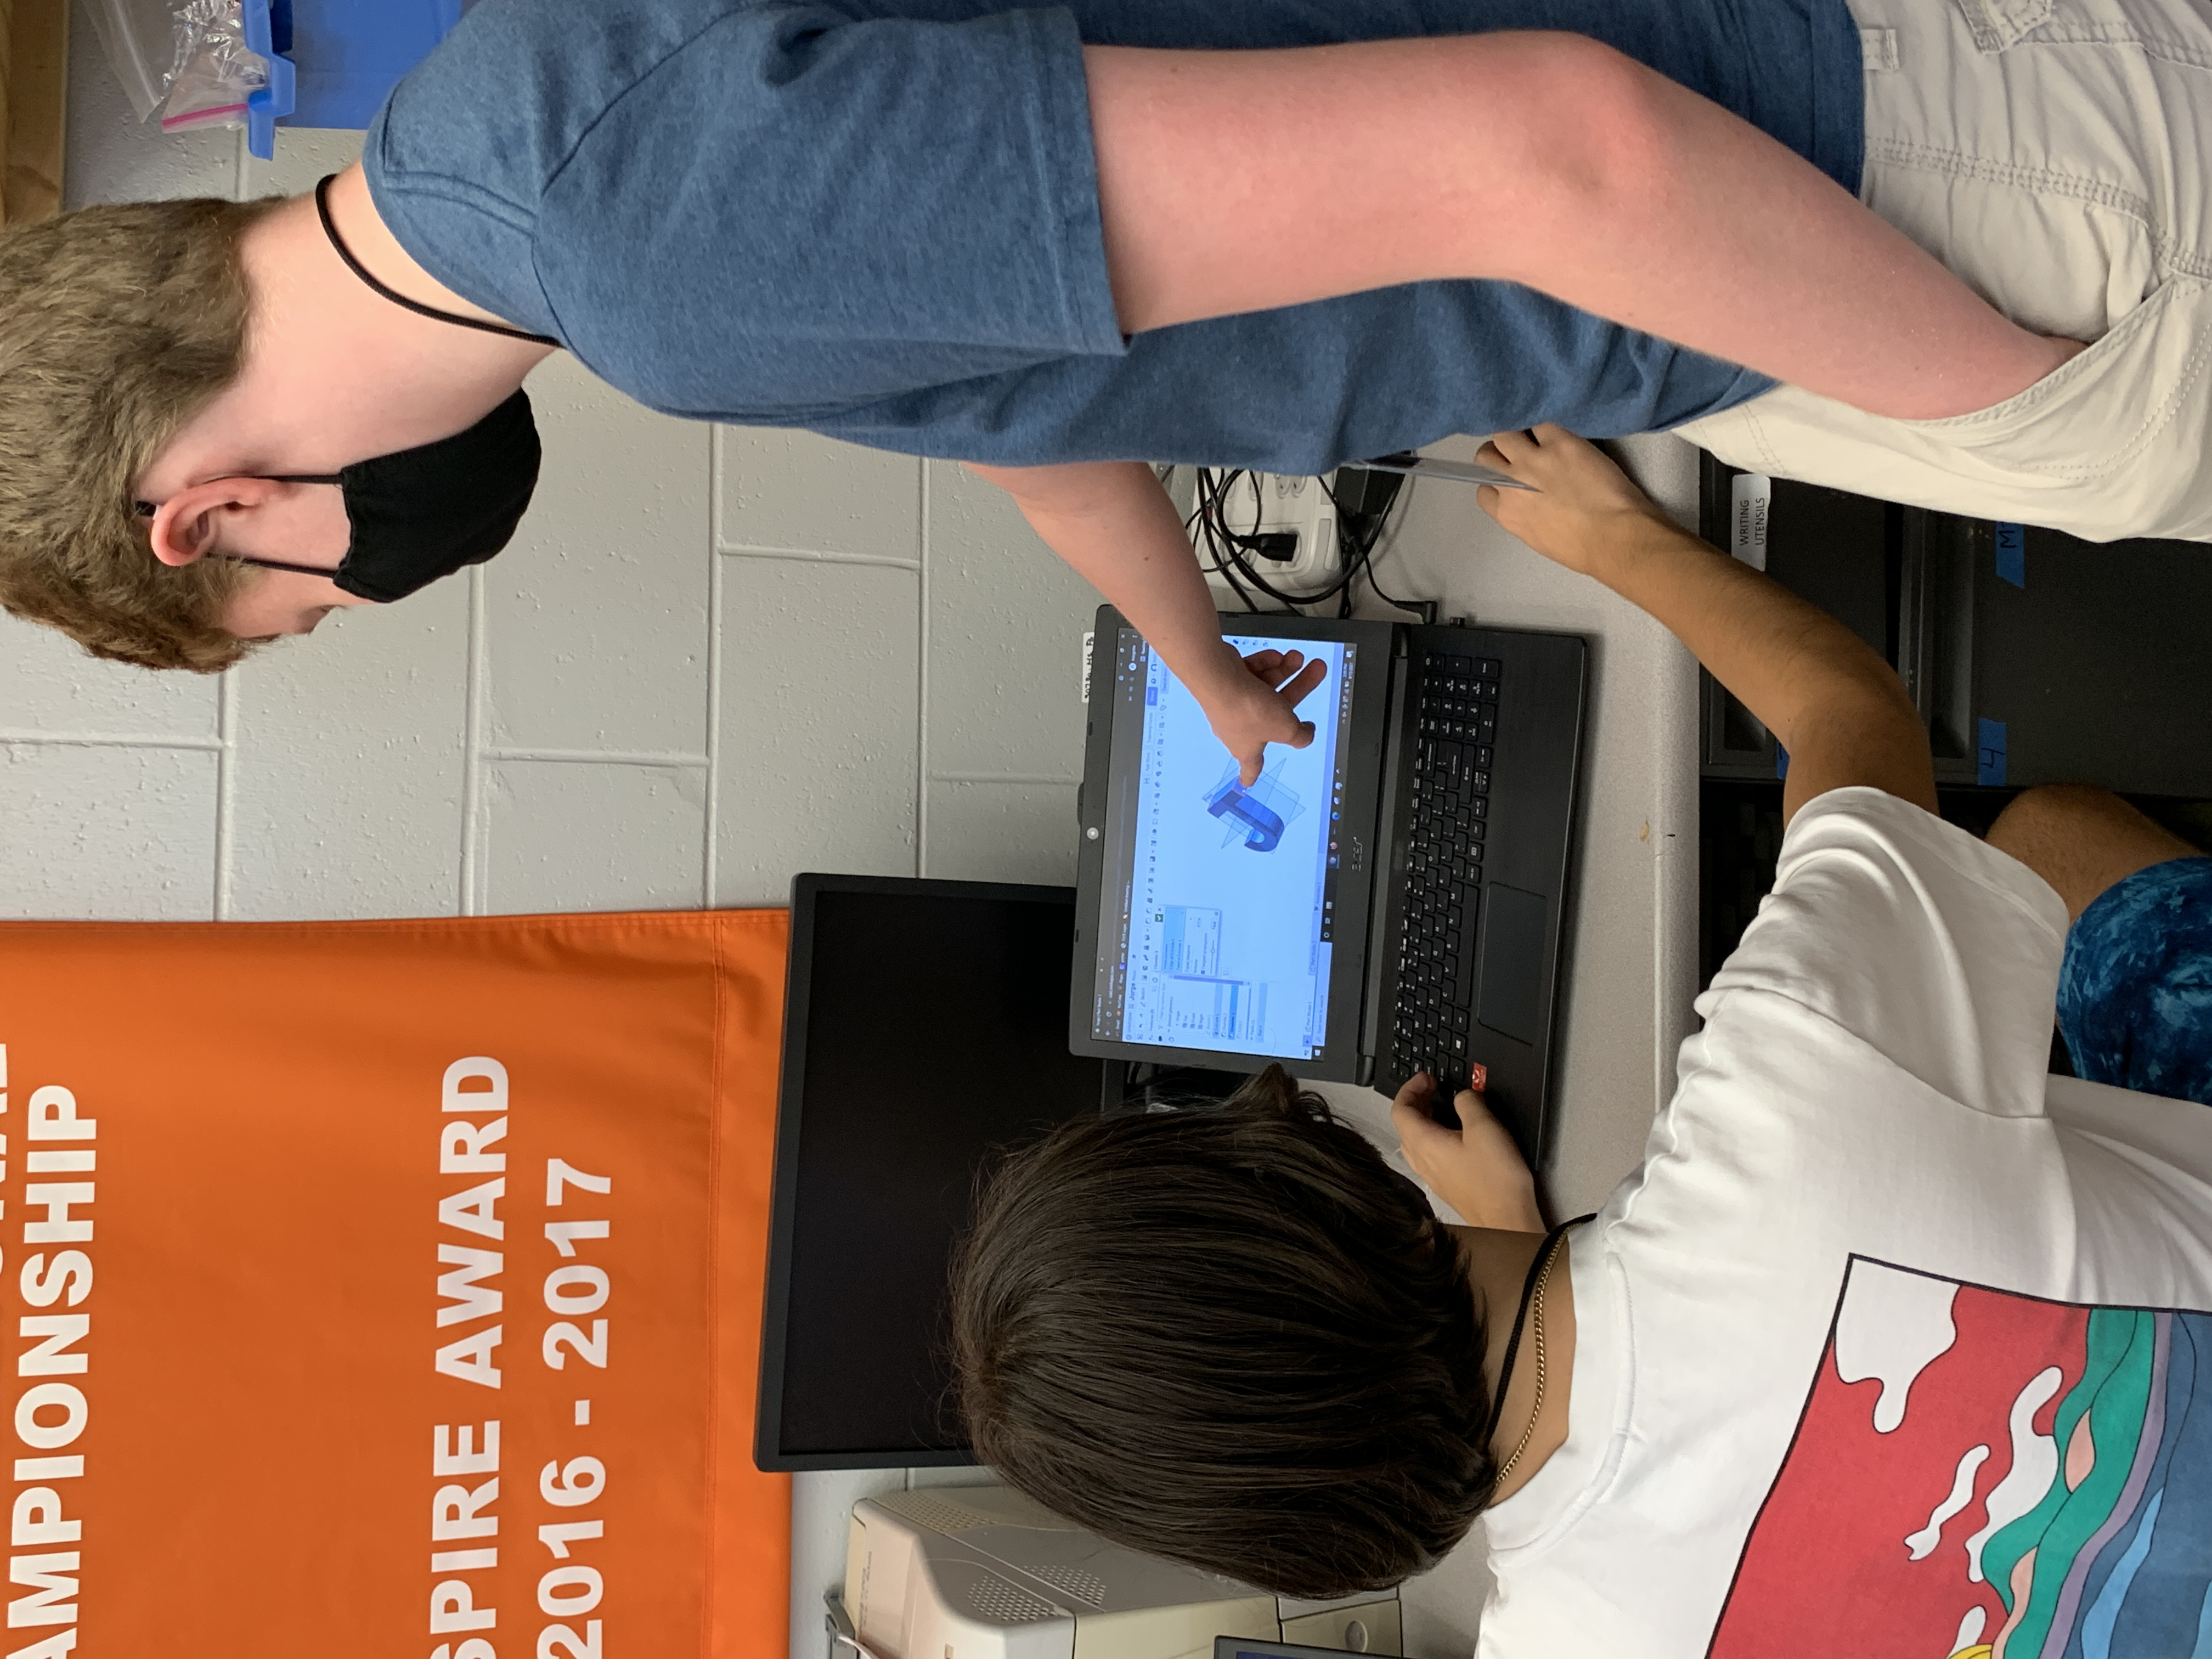
\includegraphics[width=0.8\textwidth]{Meetings/September/09-01-21/9-1-21_Program_Image2 - Nathan Forrer.JPG}
  \caption{Nathan teaching 4227 members}
  \label{fig:090121_2}
\end{minipage}
\end{figure}

\begin{figure}[htp]
\centering
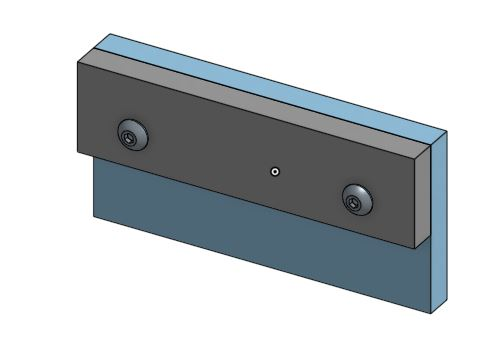
\includegraphics[width=0.8\textwidth]{Meetings/September/09-01-21/9-1-21_Program_Image3 - Nathan Forrer.JPG}
\caption{Inseritng screws}
\label{fig:090121_3}
\end{figure}


\whatsnext{
\begin{itemize}
    \item Executing the outreach we planned and working to finishing our team member takeovers so we can post them and start something else. By doing outreach, we can help others and spread awareness, but to go even further, we could send it to communications and multimedia then post about it. This will truly give us the awareness we need. Multimedia and communications still need to post some of the fun team bonding activities we had with Blue Day and Bowling. 
    \item Teach 4227 more advanced CAD
		\item Teach 4227 members software
\end{itemize} 
}






